% Options for packages loaded elsewhere
% Options for packages loaded elsewhere
\PassOptionsToPackage{unicode}{hyperref}
\PassOptionsToPackage{hyphens}{url}
\PassOptionsToPackage{dvipsnames,svgnames,x11names}{xcolor}
%
\documentclass[
]{article}
\usepackage{xcolor}
\usepackage[margin=2cm]{geometry}
\usepackage{amsmath,amssymb}
\setcounter{secnumdepth}{-\maxdimen} % remove section numbering
\usepackage{iftex}
\ifPDFTeX
  \usepackage[T1]{fontenc}
  \usepackage[utf8]{inputenc}
  \usepackage{textcomp} % provide euro and other symbols
\else % if luatex or xetex
  \usepackage{unicode-math} % this also loads fontspec
  \defaultfontfeatures{Scale=MatchLowercase}
  \defaultfontfeatures[\rmfamily]{Ligatures=TeX,Scale=1}
\fi
\usepackage{lmodern}
\ifPDFTeX\else
  % xetex/luatex font selection
\fi
% Use upquote if available, for straight quotes in verbatim environments
\IfFileExists{upquote.sty}{\usepackage{upquote}}{}
\IfFileExists{microtype.sty}{% use microtype if available
  \usepackage[]{microtype}
  \UseMicrotypeSet[protrusion]{basicmath} % disable protrusion for tt fonts
}{}
\makeatletter
\@ifundefined{KOMAClassName}{% if non-KOMA class
  \IfFileExists{parskip.sty}{%
    \usepackage{parskip}
  }{% else
    \setlength{\parindent}{0pt}
    \setlength{\parskip}{6pt plus 2pt minus 1pt}}
}{% if KOMA class
  \KOMAoptions{parskip=half}}
\makeatother
% Make \paragraph and \subparagraph free-standing
\makeatletter
\ifx\paragraph\undefined\else
  \let\oldparagraph\paragraph
  \renewcommand{\paragraph}{
    \@ifstar
      \xxxParagraphStar
      \xxxParagraphNoStar
  }
  \newcommand{\xxxParagraphStar}[1]{\oldparagraph*{#1}\mbox{}}
  \newcommand{\xxxParagraphNoStar}[1]{\oldparagraph{#1}\mbox{}}
\fi
\ifx\subparagraph\undefined\else
  \let\oldsubparagraph\subparagraph
  \renewcommand{\subparagraph}{
    \@ifstar
      \xxxSubParagraphStar
      \xxxSubParagraphNoStar
  }
  \newcommand{\xxxSubParagraphStar}[1]{\oldsubparagraph*{#1}\mbox{}}
  \newcommand{\xxxSubParagraphNoStar}[1]{\oldsubparagraph{#1}\mbox{}}
\fi
\makeatother

\usepackage{color}
\usepackage{fancyvrb}
\newcommand{\VerbBar}{|}
\newcommand{\VERB}{\Verb[commandchars=\\\{\}]}
\DefineVerbatimEnvironment{Highlighting}{Verbatim}{commandchars=\\\{\}}
% Add ',fontsize=\small' for more characters per line
\usepackage{framed}
\definecolor{shadecolor}{RGB}{241,243,245}
\newenvironment{Shaded}{\begin{snugshade}}{\end{snugshade}}
\newcommand{\AlertTok}[1]{\textcolor[rgb]{0.68,0.00,0.00}{#1}}
\newcommand{\AnnotationTok}[1]{\textcolor[rgb]{0.37,0.37,0.37}{#1}}
\newcommand{\AttributeTok}[1]{\textcolor[rgb]{0.40,0.45,0.13}{#1}}
\newcommand{\BaseNTok}[1]{\textcolor[rgb]{0.68,0.00,0.00}{#1}}
\newcommand{\BuiltInTok}[1]{\textcolor[rgb]{0.00,0.23,0.31}{#1}}
\newcommand{\CharTok}[1]{\textcolor[rgb]{0.13,0.47,0.30}{#1}}
\newcommand{\CommentTok}[1]{\textcolor[rgb]{0.37,0.37,0.37}{#1}}
\newcommand{\CommentVarTok}[1]{\textcolor[rgb]{0.37,0.37,0.37}{\textit{#1}}}
\newcommand{\ConstantTok}[1]{\textcolor[rgb]{0.56,0.35,0.01}{#1}}
\newcommand{\ControlFlowTok}[1]{\textcolor[rgb]{0.00,0.23,0.31}{\textbf{#1}}}
\newcommand{\DataTypeTok}[1]{\textcolor[rgb]{0.68,0.00,0.00}{#1}}
\newcommand{\DecValTok}[1]{\textcolor[rgb]{0.68,0.00,0.00}{#1}}
\newcommand{\DocumentationTok}[1]{\textcolor[rgb]{0.37,0.37,0.37}{\textit{#1}}}
\newcommand{\ErrorTok}[1]{\textcolor[rgb]{0.68,0.00,0.00}{#1}}
\newcommand{\ExtensionTok}[1]{\textcolor[rgb]{0.00,0.23,0.31}{#1}}
\newcommand{\FloatTok}[1]{\textcolor[rgb]{0.68,0.00,0.00}{#1}}
\newcommand{\FunctionTok}[1]{\textcolor[rgb]{0.28,0.35,0.67}{#1}}
\newcommand{\ImportTok}[1]{\textcolor[rgb]{0.00,0.46,0.62}{#1}}
\newcommand{\InformationTok}[1]{\textcolor[rgb]{0.37,0.37,0.37}{#1}}
\newcommand{\KeywordTok}[1]{\textcolor[rgb]{0.00,0.23,0.31}{\textbf{#1}}}
\newcommand{\NormalTok}[1]{\textcolor[rgb]{0.00,0.23,0.31}{#1}}
\newcommand{\OperatorTok}[1]{\textcolor[rgb]{0.37,0.37,0.37}{#1}}
\newcommand{\OtherTok}[1]{\textcolor[rgb]{0.00,0.23,0.31}{#1}}
\newcommand{\PreprocessorTok}[1]{\textcolor[rgb]{0.68,0.00,0.00}{#1}}
\newcommand{\RegionMarkerTok}[1]{\textcolor[rgb]{0.00,0.23,0.31}{#1}}
\newcommand{\SpecialCharTok}[1]{\textcolor[rgb]{0.37,0.37,0.37}{#1}}
\newcommand{\SpecialStringTok}[1]{\textcolor[rgb]{0.13,0.47,0.30}{#1}}
\newcommand{\StringTok}[1]{\textcolor[rgb]{0.13,0.47,0.30}{#1}}
\newcommand{\VariableTok}[1]{\textcolor[rgb]{0.07,0.07,0.07}{#1}}
\newcommand{\VerbatimStringTok}[1]{\textcolor[rgb]{0.13,0.47,0.30}{#1}}
\newcommand{\WarningTok}[1]{\textcolor[rgb]{0.37,0.37,0.37}{\textit{#1}}}

\usepackage{longtable,booktabs,array}
\usepackage{calc} % for calculating minipage widths
% Correct order of tables after \paragraph or \subparagraph
\usepackage{etoolbox}
\makeatletter
\patchcmd\longtable{\par}{\if@noskipsec\mbox{}\fi\par}{}{}
\makeatother
% Allow footnotes in longtable head/foot
\IfFileExists{footnotehyper.sty}{\usepackage{footnotehyper}}{\usepackage{footnote}}
\makesavenoteenv{longtable}
\usepackage{graphicx}
\makeatletter
\newsavebox\pandoc@box
\newcommand*\pandocbounded[1]{% scales image to fit in text height/width
  \sbox\pandoc@box{#1}%
  \Gscale@div\@tempa{\textheight}{\dimexpr\ht\pandoc@box+\dp\pandoc@box\relax}%
  \Gscale@div\@tempb{\linewidth}{\wd\pandoc@box}%
  \ifdim\@tempb\p@<\@tempa\p@\let\@tempa\@tempb\fi% select the smaller of both
  \ifdim\@tempa\p@<\p@\scalebox{\@tempa}{\usebox\pandoc@box}%
  \else\usebox{\pandoc@box}%
  \fi%
}
% Set default figure placement to htbp
\def\fps@figure{htbp}
\makeatother





\setlength{\emergencystretch}{3em} % prevent overfull lines

\providecommand{\tightlist}{%
  \setlength{\itemsep}{0pt}\setlength{\parskip}{0pt}}



 


\usepackage{tikz}
\usetikzlibrary{positioning,arrows.meta,calc}
\makeatletter
\@ifpackageloaded{caption}{}{\usepackage{caption}}
\AtBeginDocument{%
\ifdefined\contentsname
  \renewcommand*\contentsname{Table of contents}
\else
  \newcommand\contentsname{Table of contents}
\fi
\ifdefined\listfigurename
  \renewcommand*\listfigurename{List of Figures}
\else
  \newcommand\listfigurename{List of Figures}
\fi
\ifdefined\listtablename
  \renewcommand*\listtablename{List of Tables}
\else
  \newcommand\listtablename{List of Tables}
\fi
\ifdefined\figurename
  \renewcommand*\figurename{Figure}
\else
  \newcommand\figurename{Figure}
\fi
\ifdefined\tablename
  \renewcommand*\tablename{Table}
\else
  \newcommand\tablename{Table}
\fi
}
\@ifpackageloaded{float}{}{\usepackage{float}}
\floatstyle{ruled}
\@ifundefined{c@chapter}{\newfloat{codelisting}{h}{lop}}{\newfloat{codelisting}{h}{lop}[chapter]}
\floatname{codelisting}{Listing}
\newcommand*\listoflistings{\listof{codelisting}{List of Listings}}
\makeatother
\makeatletter
\makeatother
\makeatletter
\@ifpackageloaded{caption}{}{\usepackage{caption}}
\@ifpackageloaded{subcaption}{}{\usepackage{subcaption}}
\makeatother
\usepackage{bookmark}
\IfFileExists{xurl.sty}{\usepackage{xurl}}{} % add URL line breaks if available
\urlstyle{same}
\hypersetup{
  pdftitle={Edge cases in the three-phase kernel},
  colorlinks=true,
  linkcolor={blue},
  filecolor={Maroon},
  citecolor={Blue},
  urlcolor={Blue},
  pdfcreator={LaTeX via pandoc}}


\title{Edge cases in the three-phase kernel}
\usepackage{etoolbox}
\makeatletter
\providecommand{\subtitle}[1]{% add subtitle to \maketitle
  \apptocmd{\@title}{\par {\large #1 \par}}{}{}
}
\makeatother
\subtitle{What \texttt{\_pattern!} / \texttt{\_fill!} actually do at the
boundaries}
\author{}
\date{}
\begin{document}
\maketitle


\subsection{Setup}\label{setup}

The three-phase kernel decomposes the column axis
\texttt{{[}cmin,\ cmax{]}} into three runs of constant active count:

\begin{longtable}[]{@{}
  >{\raggedright\arraybackslash}p{(\linewidth - 6\tabcolsep) * \real{0.1238}}
  >{\raggedright\arraybackslash}p{(\linewidth - 6\tabcolsep) * \real{0.2190}}
  >{\raggedright\arraybackslash}p{(\linewidth - 6\tabcolsep) * \real{0.3333}}
  >{\raggedright\arraybackslash}p{(\linewidth - 6\tabcolsep) * \real{0.3238}}@{}}
\toprule\noalign{}
\begin{minipage}[b]{\linewidth}\raggedright
phase
\end{minipage} & \begin{minipage}[b]{\linewidth}\raggedright
columns
\end{minipage} & \begin{minipage}[b]{\linewidth}\raggedright
\texttt{active}
\end{minipage} & \begin{minipage}[b]{\linewidth}\raggedright
rows
\end{minipage} \\
\midrule\noalign{}
\endhead
\bottomrule\noalign{}
\endlastfoot
Left ramp & \texttt{{[}cmin,\ c\_LR\ −\ 1{]}} &
\texttt{max(0,\ c\ −\ rmin\ −\ δ\_lo\ +\ 1)} &
\texttt{1,\ 2,\ …,\ active(c)} \\
Interior & \texttt{{[}c\_LR,\ c\_RR{]}} &
\texttt{Leff\ =\ δ\_hi\ −\ δ\_lo\ +\ 1} const. &
\texttt{r0\ …\ r0\ +\ Leff\ −\ 1}, stride 1 \\
Right ramp & \texttt{{[}c\_RR\ +\ 1,\ cmax{]}} &
\texttt{max(0,\ δ\_hi\ −\ c\ +\ rmax\ +\ 1)} &
\texttt{r0\ …\ r0\ +\ active\ −\ 1}, stride 1 \\
\end{longtable}

with \texttt{δ\_lo\ =\ max(O,\ cmin\ −\ rmax)},
\texttt{δ\_hi\ =\ min(O\ +\ L\ −\ 1,\ cmax\ −\ rmin)},
\texttt{c\_LR\ =\ max(cmin,\ rmin\ +\ δ\_hi)},
\texttt{c\_RR\ =\ min(cmax,\ rmax\ +\ δ\_lo)},
\texttt{r0\ =\ c\ −\ δ\_hi\ −\ rmin\ +\ 1}. Inside each phase the inner
loop walks \texttt{δ} high → low so the emitted rows ascend per column
(CSC sortedness without sort). The interior uses closed-form
\texttt{cur(c)\ =\ cur\_int\_0\ +\ Leff\ *\ (c\ −\ c\_LR)} --- column
writes are independent.

This document covers the three boundary scenarios that the kernel must
handle correctly: the empty-operator early return, the off-mesh column
tails (where \texttt{max(0,\ active)} clipping kicks in), and the
\texttt{L\ =\ length(row)\ +\ 1} boundary (where the interior phase
collapses).

\subsection{\texorpdfstring{The empty operator:
\texttt{δ\_lo\ \textgreater{}\ δ\_hi}}{The empty operator: δ\_lo \textgreater{} δ\_hi}}\label{the-empty-operator-ux3b4_lo-ux3b4_hi}

If \texttt{δ\_lo\ \textgreater{}\ δ\_hi} no offset reaches any valid row
from any valid column --- the matrix is structurally all-zero. The
kernel takes an early return:

\begin{Shaded}
\begin{Highlighting}[]
\ControlFlowTok{if}\NormalTok{ δ\_lo }\OperatorTok{\textgreater{}}\NormalTok{ δ\_hi}
    \FunctionTok{resize!}\NormalTok{(rowval, }\FloatTok{0}\NormalTok{)}
    \ControlFlowTok{for}\NormalTok{ c }\KeywordTok{in}\NormalTok{ cmin}\OperatorTok{:}\NormalTok{cmax}
\NormalTok{        colptr[c }\OperatorTok{{-}}\NormalTok{ cmin }\OperatorTok{+} \FloatTok{2}\NormalTok{] }\OperatorTok{=} \FloatTok{1}
    \ControlFlowTok{end}
    \ControlFlowTok{return}
\ControlFlowTok{end}
\end{Highlighting}
\end{Shaded}

\texttt{rowval} is shrunk to length zero, and every
\texttt{colptr{[}2..n+1{]}} is set to \texttt{1} so
\texttt{colptr{[}j+1{]}\ −\ colptr{[}j{]}\ =\ 0} (zero nonzeros) for
every column. Triggering examples:

\begin{itemize}
\tightlist
\item
  Stencil sits entirely above the row range: \texttt{O\ =\ 10,\ L\ =\ 2}
  on \texttt{row\ =\ 1:5,\ col\ =\ 1:5} gives
  \texttt{δ\_lo\ =\ 10,\ δ\_hi\ =\ 4}.
\item
  \texttt{col} and \texttt{row} are far apart with small offsets:
  \texttt{row\ =\ 1:5,\ \ \ col\ =\ 100:100,\ O\ =\ -1,\ L\ =\ 3} gives
  \texttt{δ\_lo\ =\ 95,\ δ\_hi\ =\ -1}.
\end{itemize}

\subsection{\texorpdfstring{Off-mesh column tails: why
\texttt{max(0,\ active)}}{Off-mesh column tails: why max(0, active)}}\label{off-mesh-column-tails-why-max0-active}

The non-empty active set lives on column range
\texttt{{[}rmin\ +\ δ\_lo,\ rmax\ +\ δ\_hi{]}}. When \texttt{col}
extends outside this range, some columns at the extremes carry no
entries (just \texttt{colptr} markers). The ramp \texttt{active}
formulas

\begin{verbatim}
active_L(c) = c − rmin − δ_lo + 1     (left ramp)
active_R(c) = δ_hi − c + rmax + 1     (right ramp)
\end{verbatim}

go \textbf{negative} in those tails: at the left, when
\texttt{c\ \textless{}\ rmin\ +\ δ\_lo}; at the right, when
\texttt{c\ \textgreater{}\ rmax\ +\ δ\_hi}. Letting
\texttt{cur\ +=\ active} with a negative \texttt{active} would corrupt
the slot counter. The fix is to clip:

\begin{Shaded}
\begin{Highlighting}[]
\NormalTok{active }\OperatorTok{=} \FunctionTok{max}\NormalTok{(}\FloatTok{0}\NormalTok{, c }\OperatorTok{{-}}\NormalTok{ rmin }\OperatorTok{{-}}\NormalTok{ δ\_lo }\OperatorTok{+} \FloatTok{1}\NormalTok{)   }\CommentTok{\# left ramp}
\NormalTok{active }\OperatorTok{=} \FunctionTok{max}\NormalTok{(}\FloatTok{0}\NormalTok{, δ\_hi }\OperatorTok{{-}}\NormalTok{ c }\OperatorTok{+}\NormalTok{ rmax }\OperatorTok{+} \FloatTok{1}\NormalTok{)   }\CommentTok{\# right ramp}
\end{Highlighting}
\end{Shaded}

For zero \texttt{active} the inner loop
\texttt{for\ i\ in\ 0:(active\ −\ 1)} is empty, no \texttt{rowval}
writes happen, \texttt{cur} is unchanged, and only \texttt{colptr} is
written (pointing to the running \texttt{cur}).

\begin{figure}[h]
\centering
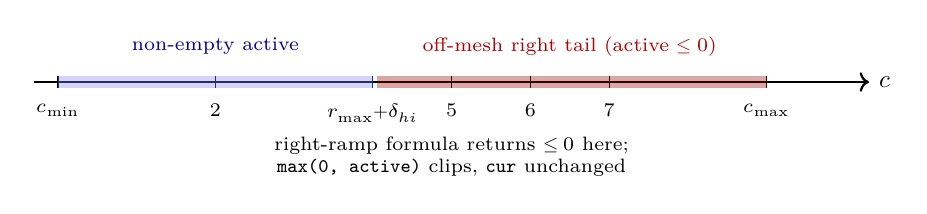
\begin{tikzpicture}[scale=1.0, font=\small]
  \draw[->, thick] (-0.3, 0) -- (10.3, 0) node[right] {$c$};

  \foreach \c/\lbl in {0/{$c_{\min}$},2/2,4/{$r_{\max}{+}\delta_{hi}$},5/5,6/6,7/7,9/{$c_{\max}$}} {
    \draw (\c, 0.08) -- (\c, -0.08);
    \node[below=2pt, font=\scriptsize] at (\c, -0.08) {\lbl};
  }

  \draw[blue!50, line width=4pt, opacity=0.35] (0, 0) -- (4, 0);
  \node[blue!60!black, font=\scriptsize] at (2, 0.45) {non-empty active};

  \draw[red!60!black, line width=4pt, opacity=0.35] (4.05, 0) -- (9, 0);
  \node[red!70!black, font=\scriptsize] at (6.5, 0.45) {off-mesh right tail (active $\le 0$)};

  \node[font=\scriptsize, align=center] at (5, -0.95)
    {right-ramp formula returns $\le 0$ here;\\\texttt{max(0, active)} clips, \texttt{cur} unchanged};
\end{tikzpicture}
\caption{Off-mesh right tail: columns past $r_{\max}+\delta_{\hi}$ produce no entries; \texttt{max(0, active)} keeps the slot counter consistent.}
\end{figure}

Concrete example:
\texttt{row\ =\ 1:5,\ col\ =\ 1:100,\ offsets\ =\ SUnitRange(-1,\ 1)}
gives \texttt{δ\_hi\ =\ 1}, so columns 7..100 lie past
\texttt{rmax\ +\ δ\_hi\ =\ 6} and the right-ramp
\texttt{active\ =\ 1\ −\ c\ +\ 5\ +\ 1} is \texttt{0,\ −1,\ −2,\ …} for
those columns.

\subsection{\texorpdfstring{The \texttt{L\ =\ length(row)\ +\ 1}
boundary}{The L = length(row) + 1 boundary}}\label{the-l-lengthrow-1-boundary}

The runtime guard \texttt{L\ −\ 1\ ≤\ length(row{[}1{]})} (= \texttt{m})
is the \emph{exact} correctness boundary of the three-phase kernel. The
interesting case is the equality \texttt{L\ =\ m\ +\ 1}.

At that boundary, with no trimming, \texttt{Leff\ =\ m\ +\ 1} and

\begin{verbatim}
c_LR − c_RR = (rmin + δ_hi) − (rmax + δ_lo) = Leff − m = 1,
\end{verbatim}

so \texttt{c\_LR\ =\ c\_RR\ +\ 1}. The interior range
\texttt{c\_LR:c\_RR} is empty (Julia handles this with a zero-iteration
\texttt{for} loop), and the left ramp covers \texttt{{[}cmin,\ c\_RR{]}}
while the right ramp covers
\texttt{{[}c\_RR\ +\ 1,\ cmax{]}\ =\ {[}c\_LR,\ cmax{]}}. The two ramps
\textbf{tile} the column range without gap.

At the last left-ramp column \texttt{c\ =\ c\_RR}, \texttt{active\ =\ m}
(the row capacity); at the first right-ramp column \texttt{c\ =\ c\_LR},
\texttt{active\ =\ m} again. The interior --- which would have wanted
all \texttt{m\ +\ 1} offsets simultaneously active --- is unreachable by
construction: no column has that much row range available.

Beyond the boundary (\texttt{L\ =\ m\ +\ 2}),
\texttt{c\_LR\ \textgreater{}\ c\_RR\ +\ 1}, and the columns in
\texttt{(c\_RR,\ c\_LR)} would need a fourth \textbf{saturated middle}
phase with both bounds dynamic and \texttt{active\ =\ m}. That phase is
deliberately out of scope; the runtime guard prevents callers from
entering this regime.

\subsection{\texorpdfstring{Why \texttt{cur} stays consistent across all
three
cases}{Why cur stays consistent across all three cases}}\label{why-cur-stays-consistent-across-all-three-cases}

The kernel maintains the invariant
\texttt{cur\ ==\ total\ nonzeros\ written\ so\ far} at every column
boundary. Each of the boundary scenarios above preserves the invariant:

\begin{itemize}
\tightlist
\item
  \textbf{Empty operator}: \texttt{cur\ =\ 1} throughout;
  \texttt{colptr} filled with \texttt{1}s.
\item
  \textbf{Off-mesh tail} (clipped \texttt{active\ =\ 0}): inner loop
  empty; \texttt{cur\ +=\ 0};
  \texttt{colptr{[}c\ −\ cmin\ +\ 2{]}\ =\ cur}.
\item
  \textbf{\texttt{L\ =\ m\ +\ 1} boundary} (empty interior): interior
  loop has zero iterations;
  \texttt{cur\ =\ cur\_int\_0\ +\ Leff\ *\ max(0,\ c\_RR\ −\ c\_LR\ +\ 1)\ =\ \ \ cur\_int\_0\ +\ 0}.
  The \texttt{max(0,\ …)} is needed because
  \texttt{c\_RR\ −\ c\_LR\ +\ 1} is \texttt{0} (range is
  \texttt{c\_LR:c\_RR\ =\ c\_LR:(c\_LR\ −\ 1)}, empty).
\end{itemize}

Together, these three mechanisms --- early return,
\texttt{max(0,\ active)} clipping, and
\texttt{max(0,\ c\_RR\ −\ c\_LR\ +\ 1)} after the interior --- make the
kernel total over the full allowed input space
\texttt{L\ ≤\ length(row)\ +\ 1}.




\end{document}
